\chapter{A simple molecular dynamics program?}
Intro

\section{The main program}
% Deducing how a molecular dynamics program does its simulations isn't always easy from looking at source code, but most programs will follow a flow similar to the following:
Most molecular dynamics programs will follow an flow similar to the following:
\begin{itemize}[midsep]
    \renewcommand{\labelitemii}{$\bullet$} % Set list depth 2 bullet thing equal to first
    \item Initialize the system. Set up the initial positions and velocities for all atoms, either by generating them or loading a saved state from a previous simulation.\todo{remove drift!}
    \item For each timestep
    \begin{itemize}[midsep]
        \item Calculate the forces between the atoms.
        \item Integrate Newton's equations of motion using an appropriate integration scheme \todo{examples?}.
        \item Sample the values of the quantities we want to study, and add to the averages.
    \end{itemize}
    \item After all timesteps have been finished we print out the measured quantities, and we could also save the state of the system so we can continue from this state later.
\end{itemize}
An example of a program that implements the above procedure can be seen in \cref{list:simple_md_program}.
\begin{listing}[!ht]
\begin{cppcode*}{gobble=4}
    System system = initializeSystem(parameters);
    double time = 0.0;
    double dt = 0.01;
    for (double time = 0; time < tMax; time += dt)
    {
        calculateForces(system);
        integrateEquationsOfMotion(system, dt);
        sample(system);
    }
\end{cppcode*}
\caption{
    An example of a typical implementation of a molecular dynamics program using object-oriented programming.
    \label{list:simple_md_program}
}
\end{listing}

When starting a new simulation we usually initialize the positions of the atoms by putting them on a regular grid like a face-centered cubic (fcc), a body-centered cubic (bcc), or a simple cubic grid. The purpose of this is to not have any atoms too close to each other, which we see from the $r^{-12}$ term would give very big forces\todo{not defined yet... move this section?}, and to start with the atoms in a state from which we are able to quickly get to the state we want to study. If we for example want to study a liquid argon system, it is wise to start in an unstable crystal state, by for example using a low density or high temperature, so that the system would melt spontaneously when we start the simulation.

\section{Calculation of forces}
The forces are calculated from the derivatives of interatomic potentials, that depend on the positions of the atoms, and generally are of the form
\begin{align*}
    U(\rvec) = \sum_{i<j} U_{ij}(r_{ij}) + \sum_{i<j<k} U_{ijk}(\rvec_i, \rvec_i, \rvec_k) + \dots,
\end{align*}
where $\rvec_i$ is the position of atom $i$, $r_{ij}$ is the distance between atom $i$ and $j$, $U_{ij}$ is a two-particle potential depending only on the distance between two atoms, and $U_{ijk}$ is a three-particle potential that usually also depends on the angle between three atoms. Higher-order contributions are also often used\todo{ReaxFF}, but they are very demanding to evaluate numerically.

When developing potentials from quantum mechanical calculations one has to weigh the benefits of having a complex potential that models the interactions accurately, against having a less comples potential that will be easier to implement, and faster to evaluate. The limiting factor in any molecular dynamics calculation is the cost of doing simulations on high-performance computing clusters\hl{like abel}, but luckily it seems like the progress in \hl{CPU} development still seems to follow Moore's Law\hl{source?}, that states that the number of transistors on integrated circuits double approximately every two years\cite{moore1965cramming}, effectively halving the price of doing a computation\hl{source?}.

In this example we will be using a potential first seen as early as 1924\cite{jones1924potential} called the Lennard-Jones potential, \hl{after its creator}. The potential is a simple two-particle potential with the following form
% To model a simple mono-atomic system we use the well-known Lennard-Jones potential\cite{jones1924potential}, which when applied on the noble gas \hl{(inert)} Argon gives results that are in good agreement with experimental results. The potential is usually written as follows
\begin{align}
%     U(r) = 4\varepsilon \Big[
%     \underbrace{
%         \left(\frac{\sigma}{r}\right)^{12}
%     }_{\text{attraction}}
%      - 
%     \underbrace{
%         \left(\frac{\sigma}{r}\right)^6
%     }_{\text{repulsion}}
%     \Big],
    U(r_{ij}) = 4\varepsilon\left[ \left(\frac{\sigma}{r}\right)^{12} - \left(\frac{\sigma}{r}\right)^{6} \right]
    = \varepsilon\left[ \left(\frac{r_m}{r}\right)^{12} - 2\left(\frac{r_m}{r}\right)^{6} \right],
    \label{eq:lennard-jones_potential}
\end{align}
where $\sigma$ is the distance between where the potential is zero \hl{(the equilibrium distance between the atoms)}, $\varepsilon$ is related to the strength of the potential (the minimum value of the potential), and $r_m = 2^{1/6} \sigma$ is the distance where the potential is at its minimum. The $r^{-12}$ term is a repulsive term that describes \hl{Pauli repulsion/steric repulsion/overlap of electron orbitals} and the $r^{6}$ term is an attractive term that describes \hl{long range/van der Waals/dipole-dipole/dispersion} interactions. \todo{something about physical justification, use 6 for repulsive because $r^{12} = (r^6)^2$}. 

The potential was used by Lennard-Jones to study the \hl{noble gas} Argon, and has been used by many others\todo{to study what? Examples}. See \cref{fig:lennard-jones_potential} for a plot of the potential using the parameters usually used for simulating Argon\cite{frenkel2001understanding}, $\sigma = 3.405$~\AA\ and $\varepsilon = 0.010318$~eV.
\begin{figure}[!ht]
    \centering
    \includesvg[width=0.7\textwidth, svgpath=./images/lennard-jones/]{lennard-jones_manualalign}
%     \includesvg[width=0.7\textwidth, svgpath=./images/lennard-jones/]{lennard-jones}
    \caption{
        Plot of the Lennard-Jones potential, as stated in \cref{eq:lennard-jones_potential}. Using the parameters usually used for simulating Argon\cite{frenkel2001understanding}, $\sigma = 3.405$~\AA\ and $\varepsilon = 0.010318$~eV.
        \label{fig:lennard-jones_potential}
    }
\end{figure}

\subsection{Newton's third law}
When calculating two-particle forces like the Lennard-Jones potential there is a simple optimization that lets us halve the number of computations, by utilizing Newton's third law. We see that when evaluating $U(r_{ij})$, the force will have the same magnitude if we switch particle $i$ and $j$. This means that when we have calculated the force $\vec F_{ij}$, from particle $j$ on particle $i$, we know that the force on atom $j$ from particle $i$ will have the same magnitude, and we can simply add the opposite force to atom $j$, $\vec F_{ji} = -\vec F_{ij}$. This way we only have to calculate the forces between particle $i$ and particles $j>i$ in the main force loop.

See \cref{list:calculate_forces,list:calculate_force_between_atoms} for an example of how to implement force calculation using the Lennard-Jones potential, using the optimization from Newton's third law.
\begin{listing}[!ht]
% \begin{cppcode*}{gobble=4}
%     void calculateForces(System &system)
%     {
%         for (Atom *atom1 : system.atoms())
%         {
%             for (Atom *atom2 : system.atoms())
%             {
%                 
%             }
%         }
%     }
% \end{cppcode*}
%         for (vector<Atom*>::iterator atom1 = atoms.begin(); atom1 != atoms.end(); ++atom1)
\begin{cppcode*}{gobble=4}
    void calculateForces(System &system)
    {
        const vector<Atom*> &atoms = system.atoms();
        for (auto atom1 = atoms.begin(); atom1 != atoms.end(); ++atom1)
        {
            // Use Newton's third law to skip half the force calculations
            for (auto atom2 = atom1.next(); atom2 != atoms.end(); ++atom2)
            {
                calculateForceBetweenTwoAtoms(*atom1, *atom2);
            }
        }
    }
\end{cppcode*}
\caption{
%     An example of how to implement the velocity Verlet integration scheme using \cpp-like object-oriented programming.
    Caption.
    \label{list:calculate_forces}
}
\end{listing}
\begin{listing}[!ht]
\begin{cppcode*}{gobble=4}
    vec3 calculateForceBetweenTwoAtoms(Atom *atom1, Atom *atom2)
    {
        vec3 drVec = atom1->position() - atom2->position();
        
        double dr2 = drVec.lengthSquared();
        double dr6 = dr2*dr2*dr2;

        double LJforce = 24.0*(2.0 - dr6)/(dr6*dr6*dr2);
        vec3 force = drVec*LJforce;
        
        atom1->force() += force;
        atom2->force() -= force; // Newton's third law
        
        return force;
    }
\end{cppcode*}
\caption{
%     An example of how to implement the velocity Verlet integration scheme using \cpp-like object-oriented programming.
    Caption.
    \label{list:calculate_force_between_atoms}
}
\end{listing}

\section{Integration scheme}
To integrate the Newton's equations of motion for the intermolecular potential there are a lot of different methods to choose between, ranging from the simple forward Euler method\hl{cite} first described by Leonard Euler in 1768, to higher order predictor-corrector methods\hl{cite}. 

It turns out that a deceptively simple method first described by Loup Verlet in 1967\cite{verlet1967computer} often satisfies our needs in an integrator, being both very accurate over long simulation times, having a \hl{global/accumulated} error of the order $\mathcal{O}(\Delta t^2)$\todo{either \cite{thijssen1999computational} sec. 8.4.1-8.4.3 or \cite{frenkel2001understanding} sec. 4.3.3, or derive self in appendix}., and numerically cheap \hl{(compared to other methods)} \hl{requiring on the order of $N$?? flops}. The Verlet method has many variations, but the simplest form \hl{(the one used/described by Verlet)} has the form
\begin{align}
    \rvec(t + \Delta t) \approx 2\rvec(t) - \rvec(t - \Delta t) + \avec(t)\Delta t^2,
    \label{eq:regular_verlet}
\end{align}
where $\Delta t$ is the timestep\todo{define timestep}, and $\avec(t)$ is the velocity at time $t$. This form of the scheme has a truncation error in the position for one timestep of the order $\mathcal{O}(\Delta t^4)$ \hl{show this}.

The stability and \hl{versatiliy} of the \hl{velocity} Verlet method comes from the fact that the scheme is symplectic\todo{show this?, appendix material}. \hl{write more about this, what this means}.

We see that the velocity isn't explicitly calculated or used in this form of the sceme, but if we need it for our experiments we can estimate the velocity using a Taylor expansion around $\rvec(t\pm\Delta t)$, which gives
\begin{align*}
    \vvec(t) = \frac{\rvec(t + \Delta t) - \rvec(t - \Delta t)}{2\Delta t},
\end{align*}
which has a truncation error for one timestep of the order $\mathcal{O}(\Delta t^2)$ \hl{show this}. 

The implementation of the Verlet scheme is mostly straightforward, the only thing we have to take care of happens in the first step. When calculating the positions in the first step, $\rvec(0+\Delta t)$, we see from \cref{eq:regular_verlet} that we need the positions from the previous step, $\rvec(0-\Delta t)$. These positions are usually \hl{simply} approximated using the initial velocity, as follows\todo{is this bad?}
\begin{align*}
    \rvec(0-\Delta t) = \rvec(0) - \vvec(0)\Delta t.
\end{align*}
See \cref{list:regular_verlet} for an example of how to implement the Verlet integration scheme.

\begin{listing}[!ht]
\begin{cppcode*}{gobble=4}
    void integrateEquationsOfMotion(System &system, double dt)
    {
        for (Atom *atom : system.atoms())
        {
            vec3 newPosition = 2.0*atom->position() - atom->oldPosition() 
                               + atom->force()*dt*dt;
            atom->oldPosition() = atom->position();
            atom->position() = newPosition;
            atom->velocity() = (atom->position() - atom->oldPosition())
                               /(2.0*dt);
        }
    }
\end{cppcode*}
\caption{
%     An example of how to implement the velocity Verlet integration scheme using \cpp-like object-oriented programming.
    Caption.
    \label{list:regular_verlet}
}
\end{listing}

The most used form of the Velocity integration scheme is called the velocity Verlet method\cite{swope1982computer}, and it has the form
\begin{align}
    \rvec(t + \Delta t) &= \rvec(t) + \vvec(t)\Delta t + \avec(t)\frac{\Delta t^2}{2}, \label{eq:velocity_verlet_position}\\
    \vvec(t + \Delta t) &= \vvec(t) + \big[\avec(t) + \avec(t + \Delta t)\big] \frac{\Delta t}{2}, \label{eq:velocity_verlet_velocity}
\end{align}
with the truncation error for one timestep $\Delta t$ being of the order $\mathcal{O}(\Delta t^3)$ for both the position and the velocity, and the \hl{global/accumulated} error being of the order $\mathcal{O}(\Delta t^2)$\hl{cite/show equivalent to regular Verlet}. 

One advantage of this form is that it is self-starting. In the regular Verlet algorithm we need $\rvec(t-\Delta t)$ to compute $\rvec(t+\Delta t)$, which we don't have at $t = 0$. This means that we have to approximate $\rvec(-\Delta T)$ somehow. In the velocity form of the algorithm we only need the positions, velocities and forces at time $t$ to calculate $\rvec(t+\Delta)$.

\hl{Show that it's equivalent to regular Verlet? to rationalize that the accumulated error is the same?}

The velocity Verlet algorithm is usually rewritten in the following way, \hl{to optimize the implementation on a computer}. We see that the new velocities can be written as
\begin{align}
    \vvec(t+\Delta t) = \tilde\vvec(t + \tfrac{1}{2}\Delta t) + \avec(t+\Delta t)\frac{\Delta t}{2}, \label{eq:verlet_velocity_with_halfstep}
\end{align}
where
\begin{align}
    \tilde\vvec(t + \tfrac{1}{2}\Delta t) = \vvec(t) + \avec(t)\frac{\Delta t}{2}.\label{eq:verlet_halfstep}
\end{align}
We see that \cref{eq:verlet_halfstep} can be used in updating the positions, so we rewrite \cref{eq:velocity_verlet_position} to
\begin{align}
    \rvec(t + \Delta t) &= \rvec(t) + \tilde\vvec(t+\tfrac{1}{2}\Delta t)\Delta t.\label{eq:velocity_verlet_positions_halfstep}
\end{align}
Which leads us to the usual way of implementing the algorithm\cite{allen1989computer}:
\begin{itemize}
    \item Calculate the velocities at $t+\tfrac{1}{2}\Delta t$ using \cref{eq:verlet_halfstep} \hl{(repeated here)}
    \begin{align*}
        \tilde\vvec(t + \tfrac{1}{2}\Delta t) = \vvec(t) + \frac{\Fvec(t)}{m}\frac{\Delta t}{2}.
    \end{align*}
    \item Calculate the new positions at $t + \Delta t$ using \cref{eq:velocity_verlet_positions_halfstep} \hl{(repeated here)}
    \begin{align*}
        \rvec(t + \Delta t) &= \rvec(t) + \tilde\vvec(t+\tfrac{1}{2}\Delta t)\Delta t.
    \end{align*}
    \item Calculate the new forces $\Fvec(t+\Delta t)$/\hl{accelerations $\avec(t+\Delta t)$}.
    \item Calculate the new velocities at $t+\Delta t$ using \cref{eq:verlet_velocity_with_halfstep} \hl{(repeated here)}
    \begin{align*}
        \vvec(t+\Delta t) = \vvec(t + \tfrac{1}{2}\Delta t) + \frac{\Fvec(t + \Delta t)}{m}\frac{\Delta t}{2}.
    \end{align*}
\end{itemize}
This implementation minimizes the memory needs, as we only need to store one copy of $\rvec$, $\vvec$ and $\Fvec$ at all times, compared to implementing \cref{eq:velocity_verlet_position,eq:velocity_verlet_velocity} which needs to store the values of both $\Fvec(t)$ and $\Fvec(t+\Delta)$ to calculate the new velocities \hl{memory usually isn't an issue...}. \todo{maybe also more computationally efficient? flops? floating point truncation?}. 

\section{Boundary conditions}
\todo[inline]{Cite Born and Von Karman 1912? (See Comp. Sim. of Liquids p. 24 (39)}
In theory we now have a working molecular dynamics program by combining \cref{list:simple_md_program,list:calculate_forces,list:calculate_force_between_atoms,list:regular_verlet}. But if we start our simulations we will quicly see that the particles will start spreading out into space, since we haven't implemented any kind of boundary conditions. The particles that are on the surface of our initial system will feel very different forces than the one in the center, and, \hl{depending on the potential, will not behave as intended?}. When simulating bulk liquids and solids we remedy this by using periodic boundary conditions. This means that we repeat the \hl{simulation box} an infinite number of times in each direction, so that all atoms \hl{have a bulk-like environment}. Atom $l$ will then have what we call an \hl{\emph{image}/``image''} in all other neighbor boxes, with position
\begin{align}
    \rvec_l^{ijk} = \rvec_l + i*L_x + j*L_y + k*L_z,
    \label{eq:pbc_positions}
\end{align}
where $(L_x, L_y, L_z)$ is the dimensions of the box, and $(i, j, k)$ is the index of the \hl{neighbor box/periodic image box}.

The first thing we have to do to implement periodic boundary conditinos is to check if any atoms have moved outside the limits of our system after each time we update the positions. An example of how to do this can be seen in \cref{list:pbc}
\begin{listing}[!ht]
\begin{cppcode*}{gobble=4}
    double calculateDistanceSquaredUsingMinimumImageConvention(
        const vec3 &u, const vec3 &v, 
        const vec3 &systemSize, const vec3 &halfSystemSize)
    {
        vec3 dr = u - v;
        for (int dim = 0; dim < 3; dim++)
        {
            if (dr[dim] => halfSystemSize[dim]) dr -= systemSize[dim];
            else if (dr[dim] < -halfSystemSize[dim]) dr += systemSize[dim];
        }
        return dr.lengthSquared(); // Avoid calculating $\sqrt{dr^2}$
    }
\end{cppcode*}
\caption{
    Minimum image convention.
    \label{list:minimum_image_convention}
}
\end{listing}

A consequence of using periodic boundary conditions is that each atom is now affected by an infinite amount of atoms. To avoid having to do an infinite number of evaluations of the potential we \hl{therefore/thus} implement something called the \hl{\emph{minimum image convention}/``minimum image convention''} \hl{source/cite?}. This \hl{means/implies} that we only calculate the force between atom $i$ and the \hl{nearest/closest} image of each atom $j$. This can for example be implemented when calculating the distance between the atoms, when calculating the forces. To avoid having an infinite amount of copies of each atom we use \cref{eq:pbc_positions} to calculate the positions of each image if needed. See \cref{list:minimum_image_convention}
\begin{listing}[!ht]
\begin{cppcode*}{gobble=4}
    void checkBoundaryConditions(System &system, const vec3 &systemSize)
    {
        for (Atom *atom : system.atoms())
        {
            for (int dim = 0; dim < 3; dim++)
            {
                if (atom->position()[dim] < 0.0) 
                    atom->position()[dim] += systemSize[dim];
                else if (atom->position()[dim] >= systemSize[dim]) 
                    atom->position()[dim] -= systemSize[dim];
            }
        }
    }
\end{cppcode*}
\caption{
    PBC.
    \label{list:pbc}
}
\end{listing}

The use of periodic boundary conditions has some other consequences for our program. The first thing we need to consider is how to calculate the forces. In theory each atom is now affected by a force from an infinite number of numbers, since we have the image of particle $j$ in an infinte number of repeating periodic boxes. Calculating an infinite number of forces for all atoms in \hl{the periodic box} is unfeasible in a numerical experiment (in nature this infinite sum is incredibly evaluated every timestep $dt = 5.39106(32)\times 10^{-44} \text{s}$ (Planck time)), so we make an approximation where we only consider the force from atoms within the size of the box.

\hl{force calculation unnecessary} Using the Lennard-Jones potential we see that the force from the potential decays as $1/r^{12}$, meaning that the force from most atoms will be neglible. \cref{fig:lennard-jones_potential}



\todo[inline]{Minimum image convention}






\chapter{Optimizations?}

\section{Verlet- and cell-lists}
    













\chapter{AwesomeChapterName}

\section{Ensemble, observables etc.}

\orangebox{
    \begin{itemize}
        \item Measure pressure, Frenkel eq. (3.4.1) p. 52.
        \item Measure temperature, Frenkel eq. (4.1.1) and (4.1.2) p. 64
    \end{itemize}
}

To measure an observable quantity in a simulation we must be able to express it as a function of the positions, velocities and forces of the particles in the system. 

According to the equipartition principle, the average total kinetic energy $\langle E_k \rangle$ is
\begin{align*}
    \left\langle E_k \right\rangle = \left\langle \frac{1}{2}mv^2 \right\rangle = \frac{3}{2}Nk_B T,
\end{align*}
from which we can derive the temperature of the system. Here $m$ is the mass of a particle, $v$ is the speed of a particle, and $T$ is the corresponding temperature of the system.

An often used method for measuring the pressure $P$ is derived from the virial equation for the pressure, which gives
\begin{align*}
    P = \rho k_B T + \frac{1}{3V}\sum_i \sum_{j>i} \bvec F(\rvec_{ij}) \rvec_{ij},
\end{align*}
where $V$ is the volume, $\rho$ is the atom density, $\bvec F(\bvec r)$ is the force between two atoms separated by $\bvec r$, and $\rvec_{ij} = \rvec_j - \rvec_i$ is the vector between atom $i$ and atom $j$. \hl{this equation depends on the ensemble, and is only valid for micro-canonical ensemble -- project 1 FYS4460}.



\section{(Initialization) A typical experimental procedure}
When doing \hl{``experiments''} using molecular dynamics we use a procedure \hl{akin to/mimicing} that used by \hl{actual} experiments. Since the duration of the experiments we are realistically able to simulate on are of the order $10^{-9} s$ / nanoseconds or below, we have to be smart when initializing the system. This means that we should start out with the system in a configuration/state as close to the one we want to study as possible. The problem with this when simulating silica/glass is that the silica structure formed when rapidly cooling molten silica doesn't have any long-range ordering. Silica in the glass form has an amorph structure, which doesn't have any long-range ordering, but has short-range ordering ``well beyond the Si-O bond length''. This structure is hard to set up with an algorithm.

\orangebox{}{
    \begin{itemize}
        \item Remove drift!
        \item Something smart about why the small timescales doesn't matter that much, since the length scales are equally small?
        \item Short/long-range order
        \item Glass transition temperature
    \end{itemize}
    \begin{quote}
        ``
        When molten silicon dioxide SiO2 is rapidly cooled, it does not crystallize but solidifies as a glass. The geometry of the silicon and oxygen centers in glass is similar to that in quartz and most other crystalline forms of the same composition, i.e., silicon is surrounded by a regular tetrahedra of oxygen centers. The difference between the glass and the crystalline forms arise from the connectivity of these tetrahedral units. Although there is no long range periodicity in the glassy network there remains significant ordering at length scales well beyond the SiO bond length. One example of this ordering is found in the preference of the network to form rings of 6-tetrahedra.[18]
        
        The glass transition temperature of pure SiO2 is about 1475 K.
        ''
        
        \url{http://en.wikipedia.org/wiki/Silicon_dioxide#Fused_quartz}
    \end{quote}
}

To generate silica in the glass form we first create a perfect silica crystal in the crystalline form $\upbeta$-cristobalite, as see in figure \cref{fig:cristobalite} \todo{Why?}, and give the atoms a random uniformly distributed velocities with mean $\mu = 0$ and standard deviation $\sigma = \sqrt{T}$, where $T$ is the wanted temperature \hl{in MD units}. The crystal consists of corner-bonded SiO$_4$ tetrahedra, and in the perfect crystallic form all silicon atoms are bound to four oxygen atoms, and all oxygen atoms to two silicon atoms.

\begin{figure}[!ht]
    \centering
    \begin{subfigure}[c]{0.25\textwidth}
%         \begin{minipage}[c]{\textwidth}
        \includesvg[width=\textwidth, svgpath=./images/beta_cristobalite/]{beta_cristobalite_x01}
%         \end{minipage}
%         \caption{\cite{wikiCristobalite01}}
        \caption{}
        \label{fig:cristobalite01}
    \end{subfigure}
    \hspace{0.07\textwidth}
    \begin{subfigure}[c]{0.45\textwidth}
%         \begin{minipage}[c]{\textwidth}
        \includesvg[width=\textwidth, svgpath=./images/beta_cristobalite/]{beta_cristobalite_xyz01}
%         \end{minipage}
%         \caption{\cite{wikiCristobalite02}}
    \caption{}
    \label{fig:cristobalite02}
    \end{subfigure}
    \caption{
        Illustrations of the $\upbeta$-cristobalite structure, from two different views. Images from Wikipedia Commons, released to the public domain\cite{wikiCristobalite01,wikiCristobalite02}.
        \label{fig:cristobalite}
    }
\end{figure}

We then heat the system to 4500 K in steps of 700 K to melt the silica crystal. We alternate between using a thermostat to adjust the temperature and simulating with the thermostat off to let the system thermalize. The number of timesteps we used for the thermostat period is around 2 500, and for the thermalization period around 10 000. We then cool the system by doing the previous procedure in reverse.

We now have a thermalized and \hl{(hopefully)} realistic silica crystal at near room temperature. From this crystal we cut out the fracture, passivate using one of the passivation methods, and fill the fracture with water molecules, \hl{and use steepest descent}. After filling the fracture with water we need to thermalize the system again, since the energy (and thereby the temperature) changes when we remove and insert atoms.

We are now ready to do measurements.

\section{Passivation}
Since we don't take into consideration molecular bonds in the silica when removing atoms to create pores, we get dangling unsaturated bonds in the system. We rectify this by passivating the system by inserting atoms on the dangling bonds, turning them into \hl{stable} silanol groups\todo{why silanol?}.

In the passivation procedure we do some basic assumptions, based on the chemical nature of silica and water. In the thermodynamically stable form, silica should have the following properties\todo{source?}:
\begin{itemize}
    \item Silicon atoms should have tetrahedral coordination, with four oxygen atoms surrounding each silicon atom in a tetrahedral \hl{shape}. \todo{On average, not all silica will have this. Something about bonds? bonded to four oxygen atoms?}
    \item Oxygen atoms should have two silicon \hl{neighbors}\todo{not all, on average}.
    \item The Si-O distance should be in the range 1.5-1.9 pm\todo{source?} (depending on the crystalline form).
\end{itemize}

\hl{When removing atoms to create pores we don't care about these properties, which leads us to the following cases}
\begin{itemize}
    \item Silicon atoms with less than four oxygen neighbors.
    \item Oxygen atoms with one missing silicon neighbor.
    \item Silicon and oxygen atoms with no neighbors.
    \item \hl{Silicon and oxygen atoms with too many neighbors?}
\end{itemize}

\hl{When inserting oxygen and hydrogen we must make sure to inject neutrally, meaning twice as much hydrogen as oxygen (H$_2$O)}

Silicon atoms with less than four oxygen atoms bound to them get ($4-n_\text{O}$) hydroxide (OH$^-$) groups attached to them, where $n_\text{O}$ is the numer of oxygen atoms bound to the silicon. Oxygen atoms with a missing silicon neighbor get a hydrogen attached. 
% \hl{(oxygen atoms with two missing neighbors are removed)}.
% Oxygen atoms with less than two silicon atoms get ($2-n_\text{Si}$) hydrogen atom attached, where $n_\text{Si}$ is the number of silicon atoms bound to the oxygen. 

When passivating a silicon atom with missing oxygen neighbors by \hl{simply} filling in the missing atoms to complete the SiO$_4$-tetrahedra. We then put one hydrogen atom on each new oxygen atom, to avoid dangling bonds on the inserted oxygen atoms.

When passivating a oxygen atom with a missing silicon neighbor, we put one hydrogen atom on the opposite side of the oxygen atom compared to the silicon atom.

All silicon and oxygen atoms with no neighbors we remove, since they aren't really part of the silica.

To find the number of \hl{neighbors/bonds/bonded atoms} for each silicon and oxygen atom, we create what we call \emph{neigbor lists}, which is a list of atoms within a chosen radius, for each atom.

\begin{figure}[!ht]
    \centering
    \begin{subfigure}[b]{0.24\textwidth}
        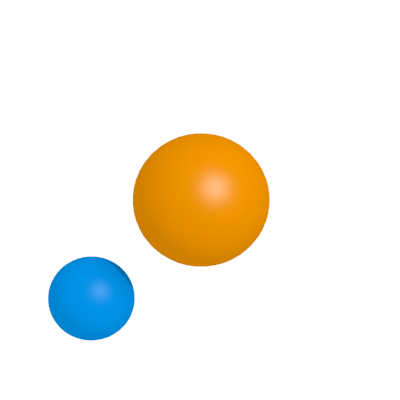
\includegraphics[width=\textwidth]{images/passivation/tetrahedra01.png}
        \caption{}
%         \caption{Illustration of how to divide a convex hexahedron into five tetraheda.}
%         \label{fig:hex_to_tetra}
    \end{subfigure}
%     \hspace{5mm}
    \begin{subfigure}[b]{0.24\textwidth}
        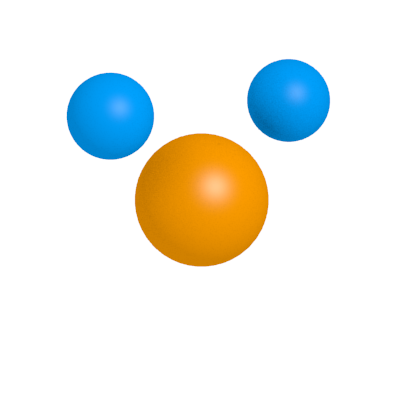
\includegraphics[width=\textwidth]{images/passivation/tetrahedra02.png}
        \caption{}
%         \caption{A random fracture made from two periodic heightmaps.}
%         \label{fig:fracture_model}
    \end{subfigure}
%     \hspace{5mm}
    \begin{subfigure}[b]{0.24\textwidth}
        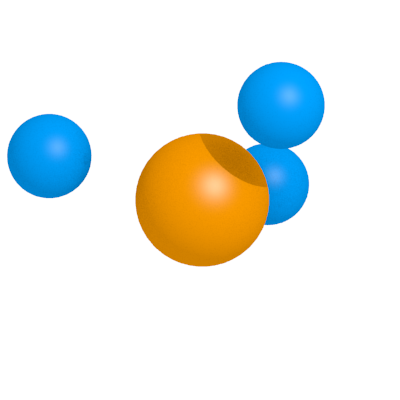
\includegraphics[width=\textwidth]{images/passivation/tetrahedra03.png}
        \caption{}
%         \caption{A random fracture made from two periodic heightmaps.}
%         \label{fig:fracture_model}
    \end{subfigure}
%     \hspace{5mm}
    \begin{subfigure}[b]{0.24\textwidth}
        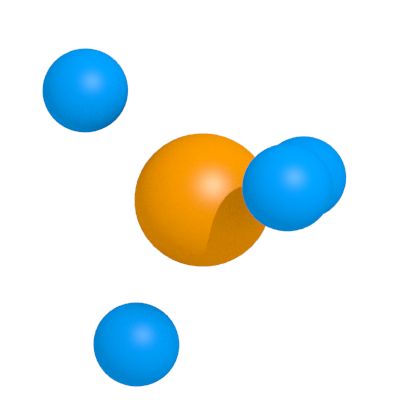
\includegraphics[width=\textwidth]{images/passivation/tetrahedra04.png}
        \caption{}
%         \caption{A random fracture made from two periodic heightmaps.}
%         \label{fig:fracture_model}\caption{}
    \end{subfigure}
    \caption{\hl{Caption}}
    \label{fig:passivation}
\end{figure}

\begin{itemize}
    \item Tetrahedra
    \item Neighbor lists -- see base\_code/passivate\_using\_tetrahedra/passivator.cpp near line 700
    \begin{itemize}
        \item Create list of atoms in each voxel
        \item Create neighbor lists for each atom by looping through neighbor voxels for each atoms
    \end{itemize}
    \item Count number of neighbors of different types -- find number of missing neighbors, Si - 4 Oxygen, Oxygen 2 Si
    \item Insert OH on Si with missing O neighbors, insert H on Oxygen with missing Si neighbors
    \begin{itemize}
        \item Insert O/H at good angles
    \end{itemize}
    \item Improvement: find the atoms near surface using voxels, only passivate those atoms
\end{itemize}

\section{Injecting water}
To fill the pore we have made \hl{(after passivating the system)} we use the technique of \emph{voxelation} (see \cref{sec:voxelation}), and put one water molecule in each unoccupied voxel. The water density is then controlled by the size of the voxels.

If we want to inject water with density $\rho$ [kg/m$^3$], we can find the voxel size we need using the molar mass of water, $M_\text{H$_2$O} = M = 0.0180158 \text{ kg/mol}$. We find the ``volume'' of a water atom in \Ang, the unit used in the \hl{MD integrator/program and output files}, as follows
\begin{align*}
    V 
    &= \frac{ M\text{ [kg/mol]} }{ \rho\text{ [kg/m$^3$]} } \\
    &= \frac{
            M\text{ [kg/mol]} \times \dfrac{1}{N_A \text{ [mol$^{-1}$]}}
        }{
            \rho\text{ [kg/m$^3$]} \times \left(10^{-10} \text{ [\AA/m]}\right)^3
        } \\
    &= \frac{M}{\rho} \times \frac{10^{-30}}{N_A} \text{ [\AA$^3$]},
%     \times \frac{N_A \text{ [mol$^{-1}$]}}{10^{-10} \text{ [\AA/m]}} 10 \text{ [m$^3$]} \\
\end{align*}
from which we find the size we need our voxels to be as
\begin{align*}
    L = \left(\frac{M}{\rho} \times \frac{10^{30}}{N_A}\right)^{1/3}\text{ [\AA]}.
\end{align*}

We then divide the system into voxels of length $L$. And put one water molecule with random orientation in the center of each empty voxel. The naive way of finding the empty voxels is to just find which voxel each existing silicon and oxygen atom is in, and mark those as occupied. But the amorph \hl{structure} of solid silica means that we have a lot of very small pores inside the matrix, which ends up as empty voxels. \todo{something about definition of a pore?}

What we do is to assign a radius to each atom type \todo{which is hard, Si-O, ???}, and mark all voxels with it's center within this radius as occupied.

\begin{itemize}
    \item Voxelize system -- size depends on wanted density
    \item Mark all voxels within distance from other atoms as occupied
    \item Fill other voxels with H2O with random O-H orientation, but correct angle
    \item Improvement: Use one voxel size in the beginning (to avoid one-voxel pores), and then use a smaller voxel size when injecting water
\end{itemize}

\section{Thermostats}
